%======================================================================
\chapter{Physics at the mesoscale}
\label{ch:swimming at the mesoscale}

\markright{Physics at the mesoscale}
%======================================================================

\section{Low Renolds Number Regime}
\label{st:lowreynoldsnumber}

At the mesoscale, where objects such as bacteria and colloidal particles operate, the physical world is governed by a regime in which viscous forces dominate over inertial ones. This regime is characterized by a small Reynolds number (Re), a dimensionless quantity that compares inertial to viscous effects. Consequently, the motion of an object at low Reynolds number is determined solely by the force acting on it at that instant; past forces have no influence on its present state. This lack of inertia is a defining feature of overdamped dynamics. In his seminal lecture, ``Life at Low Reynolds Number''~\cite{purcell2014life}, Purcell highlighted the surprising and often counterintuitive behaviors that emerge in such environments. For instance, time-reversible motion, common at macroscopic scales, is ineffective for propulsion at low Re, necessitating non-reciprocal strategies like flagellar rotation or body undulation. This leads to the scallop theorem, that states that an object with a single degree of freedom, such as a scallop in a viscous regime, will not have net displacement. 

Microswimmer dynamics can be described by the Navier–Stokes equations in the absence of inertia, reducing them to a purely viscous form without time-dependent terms, as shown in Eq.~(\ref{eq:Navier-Stokes}). This simplification reflects the highly overdamped nature of motion at the microscale. Understanding how to generate and control movement under these conditions has therefore become a central question for researchers seeking efficient propulsion and transport mechanisms at small scales. However, overcoming viscous dominance is not the only challenge faced in these environments—other factors, such as thermal fluctuations and hydrodynamic interactions, also play crucial roles.

\begin{equation}
  - \nabla p + \eta \nabla ^2 \vec{v} = 0
  \label{eq:Navier-Stokes}
\end{equation}



\section{Brownian Motion and Thermal Fluctuations}
\label{st:brownianmotion}
%%%%
Even in such a viscous regime, particles are far from motionless. At microscopic scales, like those of colloids or bacteria, random kicks from surrounding molecules constantly push them. This chaotic behavior, known as \textit{Brownian motion}, was firts give a quantitative explanation by Albert Einstein in 1905, who showed that it arises from the incessant collisions between suspended particles and the fluid's molecules~\cite{einstein1906theory}.

Einstein’s analysis did more than describe an interesting observation; it offered one of the first quantitative proofs that matter is made of atoms. From his model, he derived how the random motion of particles spreads over time, showing that the mean squared displacement (MSD) grows linearly with time:

\begin{equation}
  \expval{x^2(t)} = 2Dt, 
  \label{eq:msd}
\end{equation}

where $D$ is the duffusion coefficient, a quantity that tells how quickly a particle spreads out. Later, Einstein related $D$ to measurable properties of the system throug what is now called the \textit{Einstein-Stokes equation}.

\begin{equation}
  D = \frac{k_BT}{6\pi \eta R},
  \label{eq:diffusioncoefficient}
\end{equation}

where $k_B$ is Boltzmann's constant, $T$ the absolute temperature, $\eta$ the viscocity of the fluid, and $R$ the particle radius.

In the systems considered in this work, Brownian motion cannot be ignored since it influences the dynamics of passive colloids even when external fields or active agents are present. However, Einstein’s theory only describes the long-term diffusive behavior. To understand the instantaneous motion of a particle under both viscous drag and random forces, it is more convenient to use a stochastic approach based on the \textit{Langevin equation}.
%%%%

\subsection{Stochastic Representation}
\label{stochasticrepresentation}

The Langevin equation \cite{uhlenbeck1930theory} in one dimension, including inertial effects, damping, and thermal noise, can be written as:

\begin{equation}
  m\ddot{x} = F - \gamma \dot{x} + \eta(t)\text{,}
  \label{eq:newton}
\end{equation}

where $m$ is the particle mass, $\gamma$ is the damping coefficient, and $\eta(t)$ is a stochastic force representing thermal noise. For simplicity, we write the velocity as $v = \dot{x}$, leading to:

\begin{equation}
  m\frac{dv}{dt} = F - \gamma v + \eta(t)\text{.}
  \label{eq:newtonv}
\end{equation}

Discretizing time with a small step $dt$, we apply the definition of a derivative:

\begin{equation}
  m \frac{v(t + dt) - v(t)}{dt} = F - \gamma v(t) + \eta(t)\text{.}
  \label{eq:newtonderivative}
\end{equation}

The thermal noise term $\eta(t)$ is modeled as a Gaussian white noise process:

\begin{equation}
  \eta(t)\, dt = g\, dW\text{,}
  \label{eq:eta}
\end{equation}

where $dW$ is a Wiener increment (increment of Brownian motion) such that:

\begin{equation}
  \langle dW \rangle = 0\,, \quad \langle dW^2 \rangle = dt\text{.}
  \label{eq:meanvariance}
\end{equation}

Solving for $v(t + dt)$ gives:

\begin{equation}
  v(t + dt) = v(t) + \frac{dt}{m}(F - \gamma v(t)) + g\, dW\text{.}
  \label{eq:velocityplusone}
\end{equation}

Now, assuming no deterministic force ($F = 0$) — as is the case for free passive particles:

\begin{equation}
  v(t + dt) = v(t) - \frac{\gamma dt}{m} v(t) + g\, dW\text{.}
  \label{eq:noforce}
\end{equation}

Taking the expectation value (mean) of both sides:

\begin{equation}
  \langle v(t + dt) \rangle = \langle v(t) \rangle - \frac{\gamma dt}{m} \langle v(t) \rangle + g \langle dW \rangle\text{.}
  \label{eq:mean}
\end{equation}

Since $\langle dW \rangle = 0$, the last term vanishes:

\begin{equation}
  \langle v(t + dt) \rangle = \langle v(t) \rangle \left( 1 - \frac{\gamma dt}{m} \right)\text{.}
  \label{eq:wienerproperties}
\end{equation}

In the limit of small $dt$, this leads to the differential equation:

\begin{equation}
  \frac{d}{dt} \langle v(t) \rangle = - \frac{\gamma}{m} \langle v(t) \rangle\text{,}
  \label{eq:derivative}
\end{equation}

whose solution is:

\begin{equation}
  \langle v(t) \rangle = \langle v(0) \rangle\, e^{-\gamma t / m}\text{.}
\end{equation}

This result shows that the average velocity of a particle in a viscous fluid decays exponentially due to damping. This result describes how the velocity decays over time, depending on the mass of the particle and the dynamic drag.

%%%%

\subsection{Velocity Statistics and Energy Equipartition}

To compute the variance of the velocity, we start again from the Langevin equation in discretized form, without external forces:

\begin{equation}
  v(t + dt) = v(t) - \frac{\gamma}{m} v(t) dt + \frac{g}{m} dW \text{.}
\end{equation}

Squaring both sides:

\begin{align}
  v(t + dt)^2 &= \left[ v(t) - \frac{\gamma}{m} v(t) dt + \frac{g}{m} dW \right]^2 \text{,}\\
              &= v(t)^2 + \left( \frac{\gamma}{m} \right)^2 v(t)^2 dt^2 + \left( \frac{g}{m} \right)^2 dW^2 \nonumber \\
              &\quad - 2 \frac{\gamma}{m} v(t)^2 dt + 2 \frac{g}{m} v(t) dW - 2 \frac{\gamma g}{m^2} v(t) dW \text{.}
\end{align}

Now we take the expectation value:

\begin{align}
  \langle v(t + dt)^2 \rangle &= \langle v(t)^2 \rangle + \left( \frac{\gamma}{m} \right)^2 \langle v(t)^2 \rangle dt^2 + \left( \frac{g}{m} \right)^2 \langle dW^2 \rangle \nonumber \\
                              &\quad - 2 \frac{\gamma}{m} \langle v(t)^2 \rangle dt + 2 \frac{g}{m} \langle v(t) \rangle \langle dW \rangle - 2 \frac{\gamma g}{m^2} \langle v(t) \rangle \langle dW \rangle \text{.}
\end{align}

Using the properties of the Wiener process Eq. \ref{eq:wienerproperties}, and neglecting second-order small terms (\( dt^2 \)), we obtain:

\begin{equation}
  \langle v(t + dt)^2 \rangle = \langle v(t)^2 \rangle + \frac{g^2}{m^2} dt - 2 \frac{\gamma}{m} \langle v(t)^2 \rangle dt \text{.}
\end{equation}

Taking the continuous limit:

\begin{equation}
  \frac{d}{dt} \langle v(t)^2 \rangle = -2 \frac{\gamma}{m} \langle v(t)^2 \rangle + \frac{g^2}{m^2} \text{.}
\end{equation}

This is a linear first-order ODE. Solving it with variation of constants yields:

\begin{equation}
  \langle v(t)^2 \rangle = \frac{g^2}{2 \gamma m} + D e^{-2 \gamma t / m} \text{.}
\end{equation}

As \( t \to \infty \), the exponential term vanishes and we get the stationary value:

\begin{equation}
   \lim _{t \to \infty} \langle v(t)^2 \rangle = \frac{g^2}{2 \gamma m} \text{.}
\end{equation}

From the equipartition theorem~\cite{huang2009introduction}, we know that the average kinetic energy is:

\[
  \frac{1}{2} m \langle v^2 \rangle = \frac{1}{2} k_B T \text{.}
\]

Therefore:

\begin{equation}
  \langle v^2 \rangle = \frac{k_B T}{m} \text{.}
\end{equation}

Matching this to our stochastic result:

\begin{equation}
  \frac{k_B T}{m} = \frac{g^2}{2 \gamma m} \quad \Rightarrow \quad g^2 = 2 \gamma k_B T, \quad g = \sqrt{2 \gamma k_B T} \text{.}
\end{equation}

This defines the noise amplitude in terms of temperature, viscosity, and Boltzmann’s constant, parameters that are important when defining this type of system.

\subsection{Overdamped Dynamics and Diffussion}

In the overdamped limit, inertia is negligible, so the Langevin equation becomes:

\begin{equation}
  0 = F - \gamma \frac{dx}{dt} + \eta(t) \text{.}
\end{equation}

Solving for the velocity:

\begin{equation}
  \frac{dx}{dt} = \frac{1}{\gamma} (F + \eta(t)) \text{.}
\end{equation}

For free diffusion (\( F = 0 \)):

\begin{equation}
  \frac{dx}{dt} = \frac{1}{\gamma} \eta(t) \text{.}
\end{equation}

Using stochastic calculus with \( \eta(t) dt = g dW \), we write:

\begin{equation}
  x(t + dt) = x(t) + \frac{g}{\gamma} dW \text{.}
\end{equation}

\paragraph{Mean Position}

Taking the expectation value:

\begin{equation}
  \langle x(t + dt) \rangle = \langle x(t) \rangle + \frac{g}{\gamma} \langle dW \rangle = \langle x(t) \rangle \text{.}
\end{equation}

So the mean position remains constant in free diffusion.

\paragraph{Mean Square Displacement (MSD)}

Squaring the position update:

\begin{equation}
  x(t + dt)^2 = x(t)^2 + 2 \frac{g}{\gamma} x(t) dW + \left( \frac{g}{\gamma} \right)^2 dW^2 \text{.}
\end{equation}

Taking the expectation:

\begin{align}
  \langle x(t + dt)^2 \rangle &= \langle x(t)^2 \rangle + 2 \frac{g}{\gamma} \langle x(t) \rangle \langle dW \rangle + \frac{g^2}{\gamma^2} \langle dW^2 \rangle \text{,}\\
  &= \langle x(t)^2 \rangle + \frac{g^2}{\gamma^2} dt \text{.}
\end{align}

In differential form:

\begin{equation}
  \frac{d}{dt} \langle x(t)^2 \rangle = \frac{g^2}{\gamma^2} \text{.}
\end{equation}

Using \( g^2 = 2 \gamma k_B T \), we substitute:

\begin{equation}
  \frac{d}{dt} \langle x(t)^2 \rangle = \frac{2 k_B T}{\gamma} \text{.}
\end{equation}

Integrating gives the mean squared displacement (MSD):

\begin{equation}
  \langle x(t)^2 \rangle = \frac{2 k_B T}{\gamma} t \text{.}
\end{equation}

This is the classical diffusion result, where the diffusion coefficient is \( D = \frac{k_B T}{\gamma} \), consistent with Einstein's expression, and to better understand these dynamics, Figure~\ref{fig:passivebrowniantrajectory} helps visualize how a diffussive particle's trajectory evolves in time and its real MSD aligns with theory.



%%%%
\begin{figure}[H]
  \begin{center}
    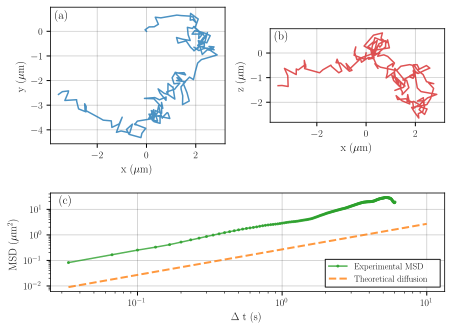
\includegraphics[width=0.8\textwidth]{figures/passivebrowniantrajectory.pdf}
  \end{center}
  \caption[Example of brownian motion]{A colloidal particle undergoes random, thermally induced displacements in a fluid medium. Panel a) and b) shows the trajectory of the particle. Panel c) shows the corresponding mean squared displacement (MSD) as a function of time, illustrating the linear relationship predicted by Einstein for diffusive behavior (orange) and the one obtained through a numerical simulation (blue).}\label{fig:passivebrowniantrajectory}
\end{figure}


